\section{Task 1: Understanding HSRN researchers' needs and behaviors}

\begin{figure}[t]
    \centering
    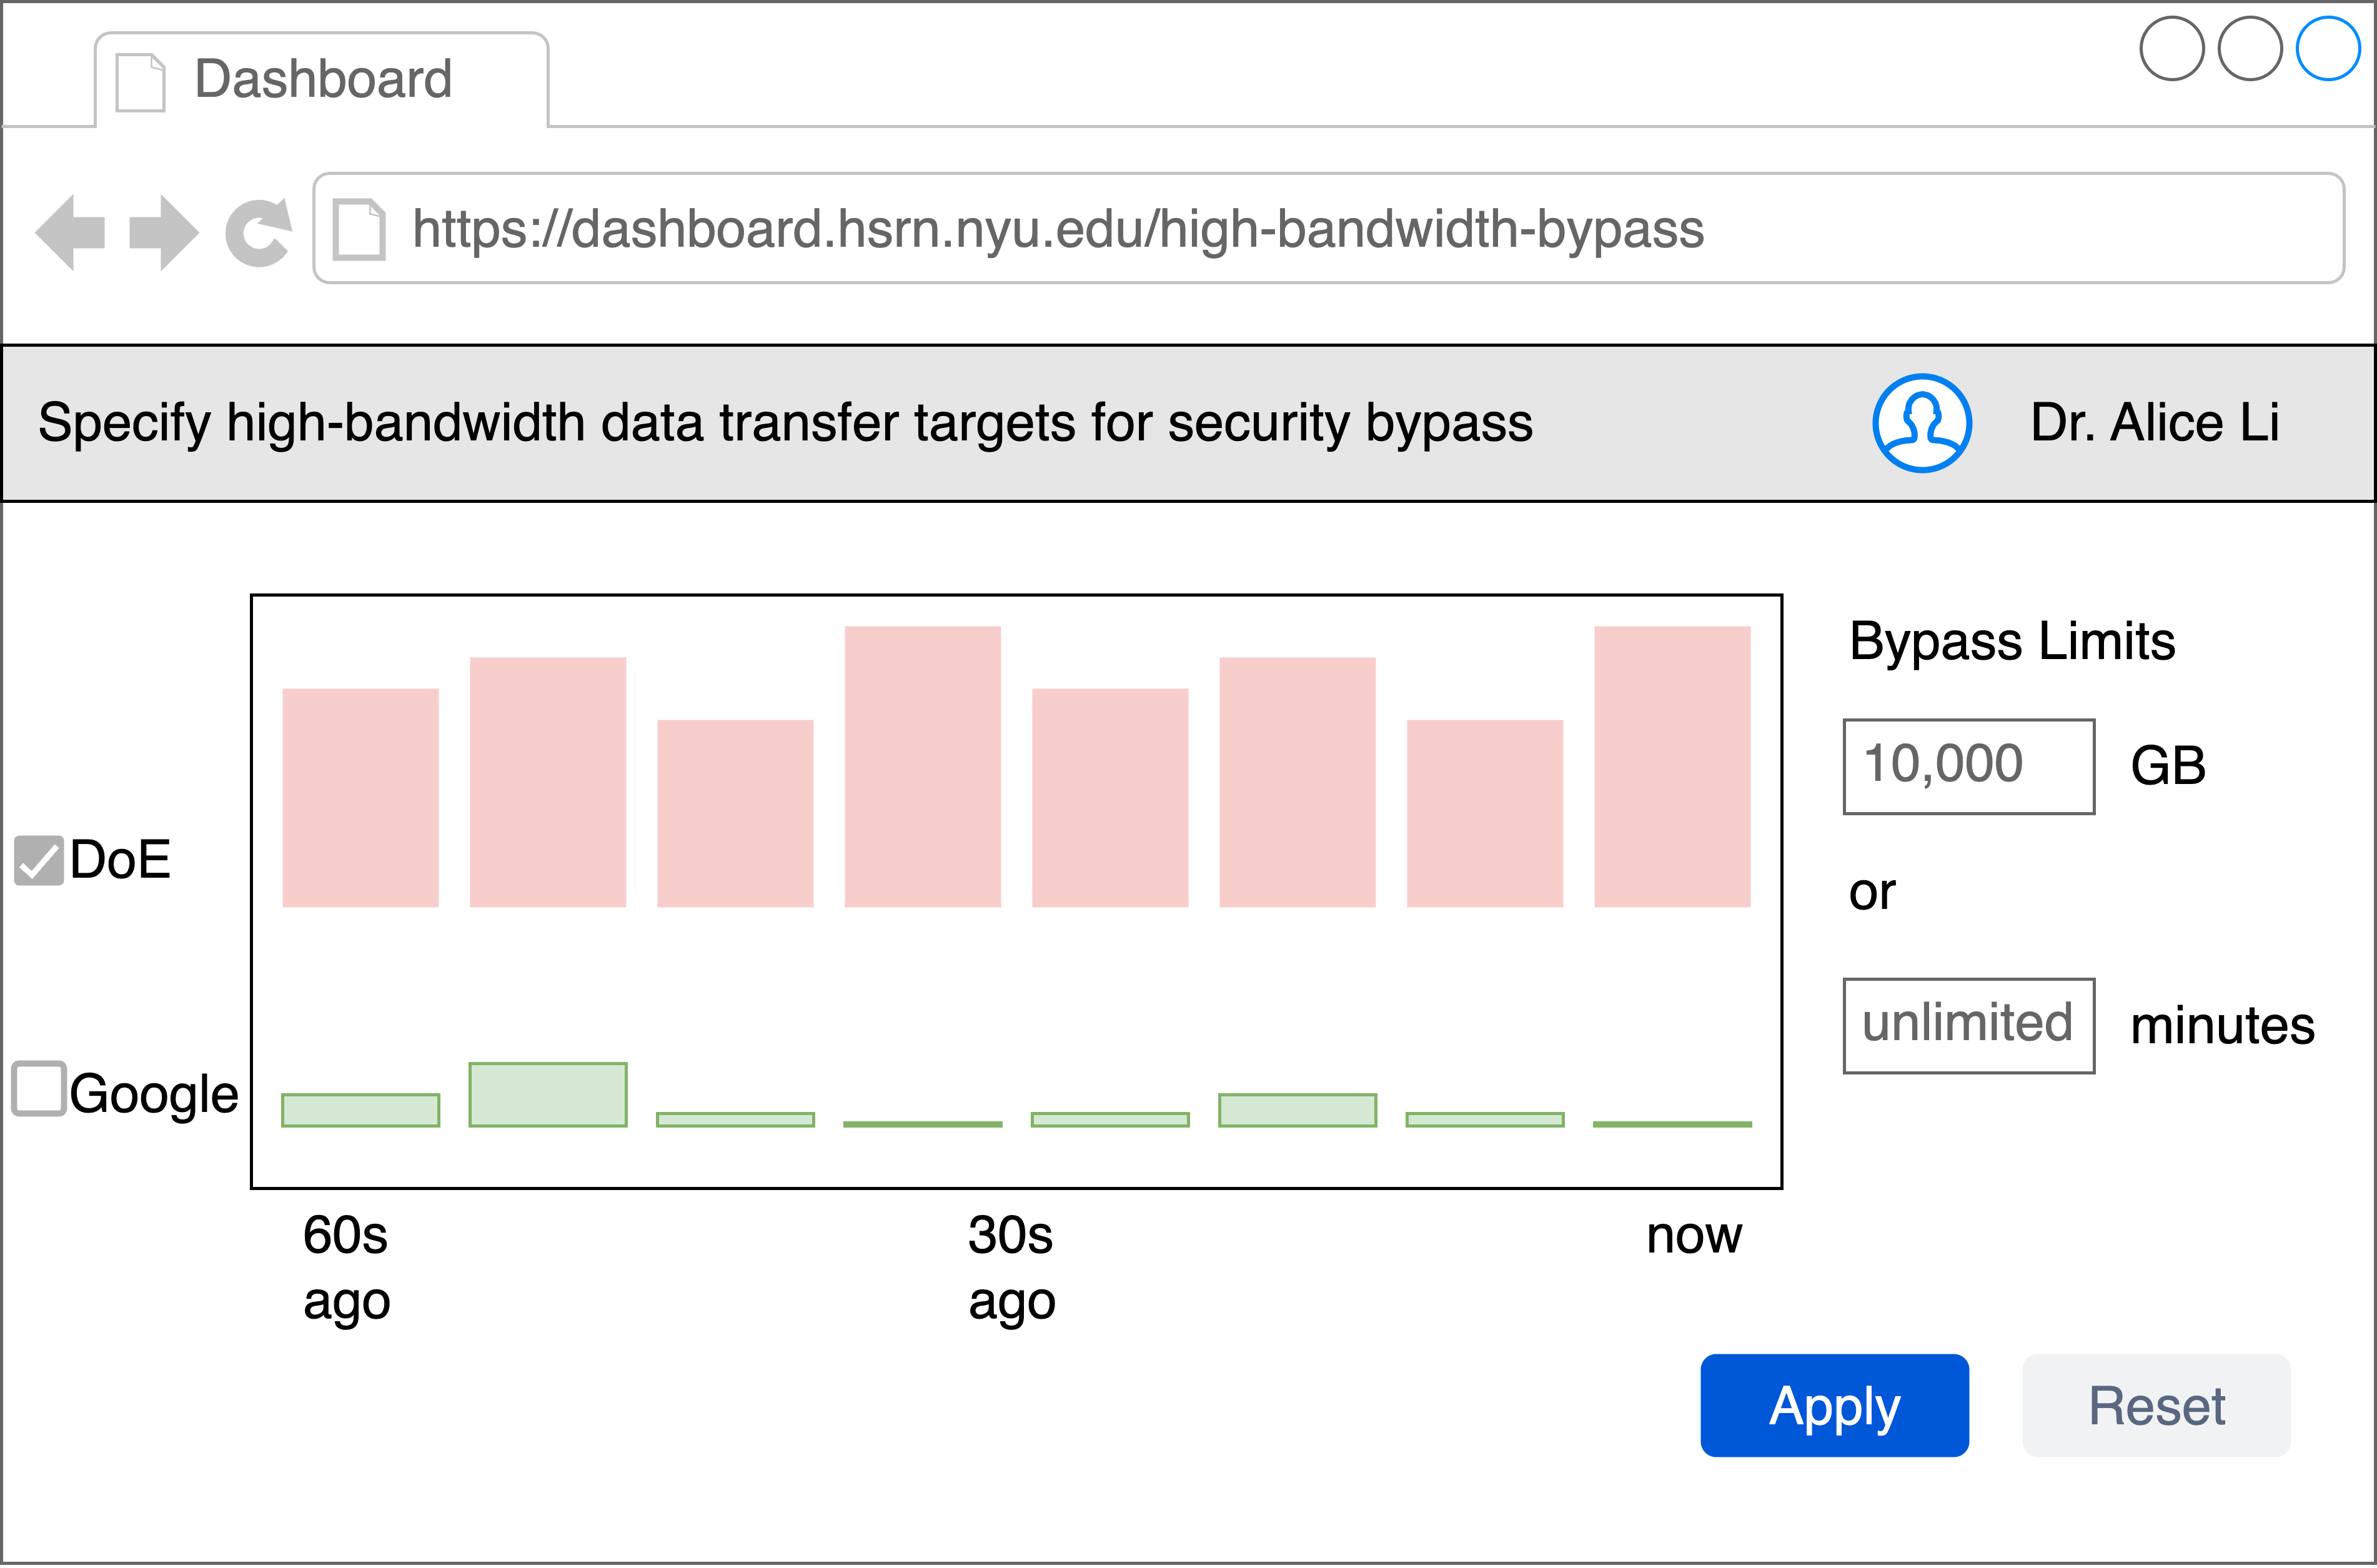
\includegraphics[width=0.5\linewidth]{figures/dashboard.png}
    \caption{A sample of the dashboard's user interface.}
    \label{fig:dashboard}
\end{figure}


Understanding researchers' needs help us design the user-facing components (UI/UX).

Understanding their behaviors help us make automated decisions to help them (especially in Task 2).

\subsection{Task 1a: Understanding researchers' needs through user studies}

\paragraph{Challenges} XXX

Understanding concerns. Through surveys and semi-structured interviews, we plan to understand how they are currently using the HSRN and their experience with the network administrators.

Co-designing UI/UX. We plan to co-design sessions in focus groups to make preliminary designs on what the dashboard looks like and the proposed user interactions. Make sure that our design is a part of their workflow.

Understand how they want to express blessed destinations or network behaviors. end-users of open scientific infrastructure may consider security processes valuable only insofar as they do not slow or otherwise impede their research

Understand qualitatively what kind of network traffic they send. Elephant flows, or latency sensitive flows, presumably depending on what kind of experiment or research work they do.

\paragraph{Preliminary work}
Inspector dashboard, CHI paper dashboard

\paragraph{Expected outcome}

// From: Jeremy
-An open source tool to monitor,visualize and manage security and data transmission in academic high speed research neworks
-A dashboard front end that  provides remote management by researchers and network administrators. .

\paragraph{Lead investigator}
PI Huang will lead the study. He's done user studies before.






\subsection{Task 1b: Identifying traffic patterns through network measurement}


\paragraph{Challenges} XXX

Clustering flows. Based on Task 1a, we know qualitatively what kinds of flows researchers tend to generate. Can we identify them? Can we cluster their network activities on the network and match against the qualitative study? For a data transfer, is it mostly elephant flows to a single destination vs mice flows? What about destinations? Let's say transfer to DoE — is it just one server, or multiple? External vs internal destinations?

\paragraph{Preliminary work} We spoke to some of the users about their work flows

// netbox already captures who is on which port and use case; flows to help us troubleshoot network speed.

no ipv6; too much work


\paragraph{Expected outcome} A measurement analysis. Clusters per researcher and type of researcher.

\paragraph{Lead investigator} Co-PI Pahle will work with IT to conduct the study, as he's already a part of the NYU research IT infrastructure team. PI Huang to help with the anonymized data analysis. PI Huang is familiar with network measurement and big data analytics.
